\documentclass[tikz,border=4pt]{standalone}
\usepackage{amsmath}
\usepackage{pgfplots}
\usepgfplotslibrary{groupplots}
\pgfplotsset{compat=1.18}
\begin{document}
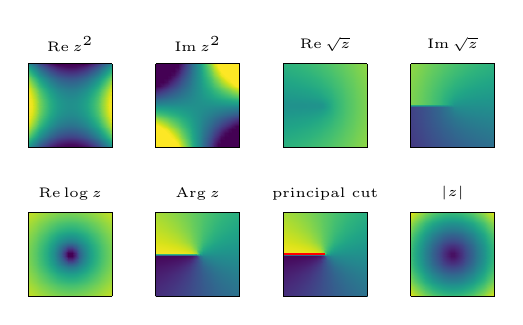
\begin{tikzpicture}
\begin{groupplot}[
  group style={group size=4 by 2,horizontal sep=0.55cm,vertical sep=0.82cm},
  width=3.15cm,height=2.65cm,
  xmin=-1.5,xmax=1.5,ymin=-1.5,ymax=1.5,
  view={0}{90},
  axis equal image,
  ticks=none,
  enlargelimits=false,
  colormap/viridis,
  point meta min=-2,
  point meta max=2,
  title style={font=\tiny,yshift=-1.2ex},
  samples=24,
  shader=interp
]
  \nextgroupplot[title={$\operatorname{Re} z^2$}]
    \addplot3[surf,domain=-1.5:1.5,y domain=-1.5:1.5] {x^2-y^2};
  \nextgroupplot[title={$\operatorname{Im} z^2$}]
    \addplot3[surf,domain=-1.5:1.5,y domain=-1.5:1.5] {2*x*y};
  \nextgroupplot[title={$\operatorname{Re}\sqrt z$}]
    \addplot3[surf,domain=-1.5:1.5,y domain=-1.5:1.5]
      {sqrt((sqrt(x^2+y^2)+x)/2)};
  \nextgroupplot[title={$\operatorname{Im}\sqrt z$}]
    \addplot3[surf,domain=-1.5:1.5,y domain=-1.5:1.5]
      {ifthenelse(y<0,-1,1)*sqrt((sqrt(x^2+y^2)-x)/2)};
  \nextgroupplot[title={$\operatorname{Re}\log z$},point meta min=-2,point meta max=1]
    \addplot3[surf,domain=-1.5:1.5,y domain=-1.5:1.5]
      {ln(max(0.06,sqrt(x^2+y^2)))};
  \nextgroupplot[title={$\operatorname{Arg} z$},point meta min=-3.2,point meta max=3.2]
    \addplot3[surf,domain=-1.5:1.5,y domain=-1.5:1.5]
      {atan2(y,x)*pi/180};
  \nextgroupplot[title={principal cut},point meta min=-3.2,point meta max=3.2]
    \addplot3[surf,domain=-1.5:1.5,y domain=-1.5:1.5]
      {atan2(y,x)*pi/180};
    \draw[red,thick] (axis cs:-1.5,0) -- (axis cs:0,0);
  \nextgroupplot[title={$|z|$},point meta min=0,point meta max=2.2]
    \addplot3[surf,domain=-1.5:1.5,y domain=-1.5:1.5]
      {sqrt(x^2+y^2)};
\end{groupplot}
\end{tikzpicture}
\end{document}
